\documentclass[conference]{IEEEtran}
\usepackage{times}

% numbers option provides compact numerical references in the text. 
\usepackage[numbers]{natbib}
\usepackage{multicol}
\usepackage[bookmarks=true]{hyperref}
\usepackage{color}
\usepackage{amsmath}
\usepackage{amssymb}
\usepackage{booktabs}
\usepackage{mathtools}
\usepackage{graphicx}
\usepackage{graphicx}
\usepackage{caption}
\usepackage{subcaption}
% Variables used across report
\newcommand{\actionset}{\ensuremath{\mathcal{A}}}
\newcommand{\actionsetsize}{\ensuremath{|\mathcal{A}|}}
\newcommand{\actionvar}{\ensuremath{a}}
\newcommand{\actionsub}[1]{\ensuremath{a_{#1}}}
\newcommand{\actionsubsup}[2]{\ensuremath{a_{#1}^{#2}}}

\newcommand{\demoset}{\ensuremath{\mathcal{D}}}
\newcommand{\demovar}{\ensuremath{d}}
\newcommand{\demosub}[1]{\ensuremath{d_{#1}}}
\newcommand{\demosubsup}[2]{\ensuremath{d_{#1}^{#2}}}

\newcommand{\trajset}{\ensuremath{\mathcal{T}}}

\newcommand{\labelset}{\ensuremath{\mathcal{L}}}
\newcommand{\labelsetsize}{\ensuremath{|\mathcal{L}|}}
\newcommand{\labelvar}{\ensuremath{\ell}}
\newcommand{\labelsub}[1]{\ensuremath{l_{#1}}}
\newcommand{\nsub}[1]{\ensuremath{n_{#1}}}
\newcommand{\sapairsub}[1]{\ensuremath{(s_{#1}, a_{#1})}}

\newcommand{\stateset}{\ensuremath{\mathcal{S}}}
\newcommand{\statevar}{\ensuremath{s}}
\newcommand{\statesub}[1]{\ensuremath{s_{#1}}}
\newcommand{\statesubsup}[2]{\ensuremath{s_{#1}^{#2}}}
\newcommand{\nextstatevar}{\ensuremath{s'}}
\newcommand{\transitionfn}{\ensuremath{T}}
\newcommand{\rewardfn}[1]{\ensuremath{R}}
\newcommand{\goalset}{\ensuremath{\mathcal{G}}}

\newcommand{\policyset}{\ensuremath{{\Pi}}}
\newcommand{\policyvar}{\ensuremath{\pi}}
\newcommand{\policysub}[2]{\ensuremath{\pi_{#1}(#2)}}

\newcommand{\regcost}{\ensuremath{r}}
\newcommand{\indexvar}{\ensuremath{i}}

\newcommand{\landmarkset}{\ensuremath{\mathcal{K}}}

\newcommand{\marginvar}{\ensuremath{m}}
\newcommand{\approxq}{\ensuremath{\tilde{Q}}}
\newcommand{\weights}{\ensuremath{w}}
\newcommand{\weightszero}{\ensuremath{w_0}}
\newcommand{\weightst}{\ensuremath{w^\intercal}}
\newcommand{\featurefn}{\ensuremath{\phi}}
\newcommand{\features}[2]{\ensuremath{\phi({#1}, {#2})}}
\newcommand{\marginslackc}{\ensuremath{C}}
\newcommand{\marginslacksubsup}[2]{\ensuremath{\xi_{#1}^{#2}}}
\newcommand{\bellmanslackc}{\ensuremath{D}}
\newcommand{\bellmanslacksubsup}[2]{\ensuremath{\nu_{#1}^{#2}}}
\newcommand{\bellmanc}{\ensuremath{F}}


\pdfinfo{
   /Author (Homer Simpson)
   /Title  (Robots: Our new overlords)
   /CreationDate (D:20101201120000)
   /Subject (Robots)
   /Keywords (Robots;Overlords)
}

\DeclareMathOperator*{\argmin}{argmin}
\DeclareMathOperator*{\argmax}{argmax}

\newcommand{\et}[1]{\textcolor{blue}{Eric: #1}}
\newcommand{\dhm}[1]{\textcolor{red}{Dylan: #1}}
\newcommand{\sh}[1]{\textcolor{green}{Sandy: #1}}
\newcommand{\al}[1]{\textcolor{magenta}{Alex: #1}}

\begin{document}
% paper title
\title{Learning to Select Expert Demonstrations for Deformable Object Manipulation}
% Learning to Use Expert Demonstrations

% You will get a Paper-ID when submitting a pdf file to the conference system
\author{Dylan Hadfield-Menell, Alex Lee, Sandy Huang, Eric Tzeng, and Pieter Abbeel}

%\author{\authorblockN{Michael Shell}
%\authorblockA{School of Electrical and\\Computer Engineering\\
%Georgia Institute of Technology\\
%Atlanta, Georgia 30332--0250\\
%Email: mshell@ece.gatech.edu}
%\and
%\authorblockN{Homer Simpson}
%\authorblockA{Twentieth Century Fox\\
%Springfield, USA\\
%Email: homer@thesimpsons.com}
%\and
%\authorblockN{James Kirk\\ and Montgomery Scott}
%\authorblockA{Starfleet Academy\\
%San Francisco, California 96678-2391\\
%Telephone: (800) 555--1212\\
%Fax: (888) 555--1212}}


% avoiding spaces at the end of the author lines is not a problem with
% conference papers because we don't use \thanks or \IEEEmembership


% for over three affiliations, or if they all won't fit within the width
% of the page, use this alternative format:
% 
%\author{\authorblockN{Michael Shell\authorrefmark{1},
%Homer Simpson\authorrefmark{2},
%James Kirk\authorrefmark{3}, 
%Montgomery Scott\authorrefmark{3} and
%Eldon Tyrell\authorrefmark{4}}
%\authorblockA{\authorrefmark{1}School of Electrical and Computer Engineering\\
%Georgia Institute of Technology,
%Atlanta, Georgia 30332--0250\\ Email: mshell@ece.gatech.edu}
%\authorblockA{\authorrefmark{2}Twentieth Century Fox, Springfield, USA\\
%Email: homer@thesimpsons.com}
%\authorblockA{\authorrefmark{3}Starfleet Academy, San Francisco, California 96678-2391\\
%Telephone: (800) 555--1212, Fax: (888) 555--1212}
%\authorblockA{\authorrefmark{4}Tyrell Inc., 123 Replicant Street, Los Angeles, California 90210--4321}}


\maketitle

%% \begin{abstract}
%% We consider the problem of learning from demonstrations
%% to manipulate deformable objects. Recent
%% work~\cite{Schulmanetal_IROS2013, Schulmanetal_ISRR2013} has shown
%% promising results in enabling robotic manipulation of deformable
%% objects through learning from demonstrations.  Their approach is able
%% to generalize from a single demonstration to new test situations,
%% and suggests a nearest
%% neighbor approach to decide which demonstration to generalize from for
%% a given test situation.  Such a nearest neighbor approach, however,
%% ignores important aspects of the problem:  brittleness (versus
%% robustness) of demonstrations when generalized through this process,
%% and the extent to which a demonstration makes progress towards the goal.

%% In this paper, we present a max-margin q-learning-based solution
%% to the demonstration selection problem that
%% can account for the variability in robustness of demonstrations and the
%% sequential nature of our tasks.   We also present experimental
%% validation of our approach.  We developed a knot-tying benchmark for
%% evaluating the effectiveness of
%% our proposed approach.   The
%% nearest neighbor approach described in \citet{Schulmanetal_ISRR2013} achieves a
%% 68.8\% success rate. Our approach achieves a success rate of 95.2\%.
%% \end{abstract}
\section{Overview}
Automated manipulation of deformable objects tends to be challenging
due to high-dimensional, continuous state-action spaces and due to the
complicated dynamics of deformable objects. Direct planning or optimal
control techniques are often intractable for this setting.

Despite these challenges, recent work~\cite{Schulmanetal_IROS2013,
  Schulmanetal_ISRR2013} has leveraged expert demonstrations to make
progress on robotic manipulation of deformable objects. This work uses
non-rigid registration between a demonstration scene and a test scene
to find a geometric mapping between the demonstration and test scene.
This mapping is used to perform \emph{trajectory transfer} for the
demonstrated gripper trajectory. This approach has been validated in
simulated and real-world environments for knot-tying, suturing, and
folding tasks.

Full demonstrations of complex tasks with multiple steps are hard
to collect and transfer successfully. As such, we assume that
demonstrations often correspond to steps in the task, rather than the
entire task itself. Figure~\ref{fig:knot_steps} shows an example of
the steps involved in tying an overhand knot. Furthermore, a single demonstration
for a step in the task cannot be expected to cover all possible
scenarios that arise during execution.  The natural solution to this
is to use a library of demonstrations with multiple demonstrations for
each step.

Realizing the benefits of a demonstration library requires a robust
technique to select a good trajectory to transfer.  Certain
trajectories will generalize better than others, and particular
sequences of demonstrations may perform tasks more efficiently than
others.

The original paper on the approach of trajectory transfer
prescribes choosing the trajectory segment from the demonstrations
library with the lowest warping cost onto the current
scene~\citep{Schulmanetal_ISRR2013}.  This approach does not account
for the inherent generalizability of a particular demonstration. For
brittle demonstrations (e.g. grabbing near the edge of a rope), a
small change in the rope can have low registration cost, but the
transferred trajectory will fail.  As a result, such an approach may
fail to accomplish tasks that would be possible with a different
sequence of trajectories.

\begin{figure}[t]
  \centering
    \noindent
    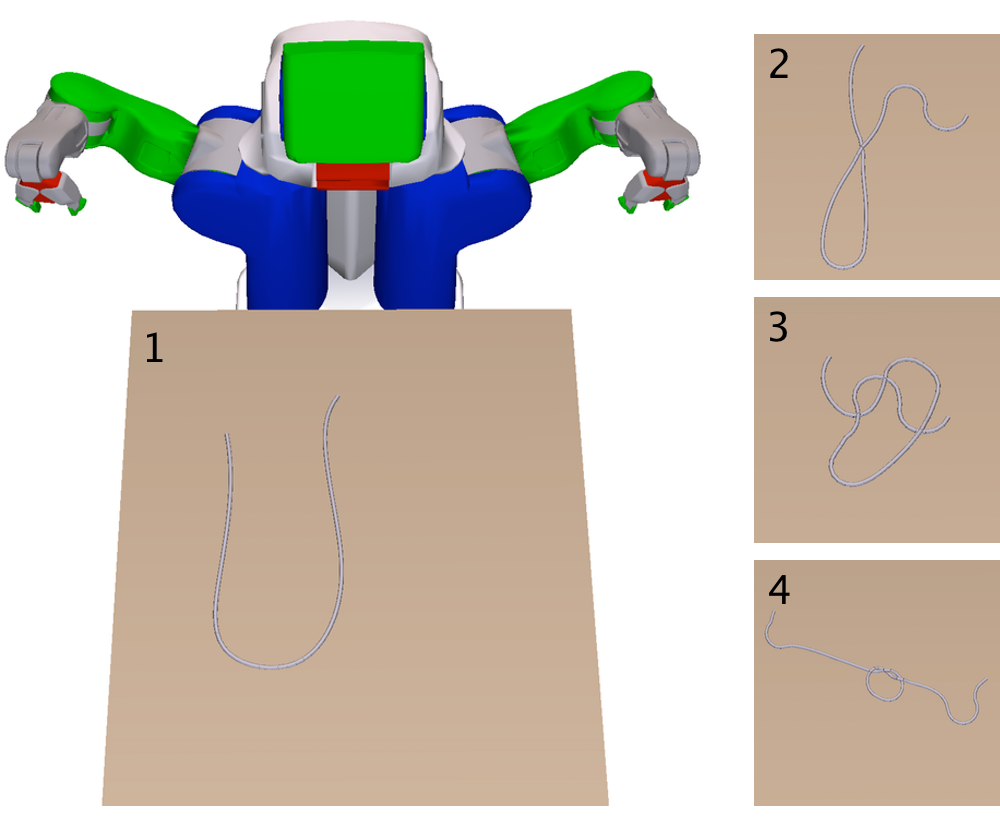
\includegraphics[width=0.45\textwidth]{figures/knot_steps_num.png}
  \caption{The overhand knot manipulation task in our benchmark.
           A standard knot tie takes three steps, as shown in this
           particular execution from our benchmark.}
  \label{fig:knot_steps}
\end{figure}

In this work, we present a solution to the demonstration selection
problem that can account for the variability in robustness of
demonstrations and incorporates the sequential nature of our
tasks. Our contributions are as follows: (i) We formulate the
demonstration selection problem as a Markov Decision Process (MDP);
(ii) We present a method for approximating $Q$-functions from
expert-guided task executions, based on the optimality of the expert's
action selection; (iii) We describe task-independent features that are
rich enough to allow learning but make no additional assumptions
beyond those of trajectory transfer; and (iv) We validate this
approach in a simulated knot-tying experiment and show strong
improvement over previous approaches.

\section{Trajectory Transfer \& MDP Formulation}

Non-rigid registration computes a function $f$ that minimizes error
between landmark points, subject to a regularization term.  A
commonly-used, effective method for registering spatial data is the
Thin Plate Spline (TPS) regularizer~\citep{Carr_SIGGRAPH2001,
  Wahba_TPS1990}.  Given a set of correspondence points
$(\mathbf{x}_i, \mathbf{y}_i)$, the goal is to find the warping
function $\mathbf{f} : \mathbb{R}^3 \rightarrow \mathbb{R}^3$ that
minimizes the following objective:
$$\min_{\mathbf{f}} \sum_i ||\mathbf{x}_i - \mathbf{y}_i||^2 + C\int
dx ||\text{D}^2(\mathbf{f})||^2_{\text{Frob}},$$ where $C$ is a
hyper-parameter that trades off between correspondence error and
increased curvature.  The second term measures curvature:
$\text{D}^2(\mathbf{f})$ is the matrix of second order partial
derivatives of $\mathbf{f}$, and $||\cdot||^2_{\text{Frob}}$ denotes
the Frobenius norm.  This problem has a finite dimensional solution in
terms of basis functions around the correspondence points.  More
concretely, $\mathbf{f}$ has the form
$$\mathbf{f}(\mathbf{x}) = \sum_i \mathbf{a}_i K(\mathbf{x}_i, \mathbf{x}) + \mathbf{B}\mathbf{x} + \mathbf{c}$$
where $K$ is the 3D TPS kernel $K(\mathbf{x}, \mathbf{x}') = - ||\mathbf{x} - \mathbf{x}'||$, and $\mathbf{a}_i \in \mathbb{R}^3$, $\mathbf{B} \in \mathbb{R}^{3\text{x}3}$, and $\mathbf{c} \in \mathbb{R}^3$.


%%SH This paragraph seems a little out of place -- maybe we should
%%   delete it? Or merge this paragraph and the following one. I like
%%   the part of this paragraph that mentions the motivation behind
%%   maximizing rigidity of the warp.
In particular, this method of trajectory transfer uses a thin- plate
spline (TPS) to find a mapping between these two scenes. A TPS
minimizes the curvature of the mapping function and tries to find a
mapping, or warping, that is close to rigid. This is motivated by the
observation that for many tasks, success in a task is preserved under
Euclidean transformation. Furthermore, the associated optimization
problem can be solved efficiently~\citep{Wahba_TPS1990}.

\citet{Schulmanetal_ISRR2013} leverage thin plate splines to perform
trajectory transfer.  Using a point cloud representation of both
scenes, they find a TPS that maps from the demonstration scene to the
new scene.  The transformation function is used to warp the path
traced by the end effector of the robot in the demonstration,
represented as a sequence of end effector poses. The warped trajectory
is executed, with the hope that the registration will account for
changes in the environment but maintain the important aspects of the
manipulation.


We consider the case where an agent has access to a library of expert
demonstrations. Such a library enables task execution from different
initial conditions and provides robustness to different types of
environmental variation. With many demonstrations, the decision making
problem is to select which demonstration trajectory to transfer.

We approach the problem of selecting a trajectory to transfer as an
abstract MDP. Our base manipulation task is an MDP with
high-dimensional, continuous state and action spaces. For a knot-tying
task, the state space is the joint state of the robot and the
rope. The action space is the set of torques that can be applied at
the motors. With a library of demonstrations, we can reduce this
problem to an abstract MDP where the state space is the same, but the
actions correspond to selecting a trajectory from the library and transferring it to
the current state. This abstracts the problem temporally and
significantly reduces the size of the action space. Actions follow a
sequence of waypoints, thus significantly reducing the time horizon to be considered.
Furthermore, because there are finitely many
demonstrations, the continuous action space is reduced to a finite
set of options.

Using this formalization, we learn an approximate Q-function for the
abstract MDP. This is still a continuous-state reinforcement learning
problem, so we propose a method to do this learning with human
input. The procedure combines maximum-margin structured prediction
with approximate linear programming to learn a $Q$-function that 1)
matches a human demonstrator's $Q$-function and 2) is consistent
with the dynamic programming equations for the MDP. 

\section{Experiments and Benchmark}

We developed a knot-tying benchmark for evaluating the effectiveness
of our proposed approach.  This benchmark is available at
\href{https://sites.google.com/site/rss2014mmql}{sites.google.com/site/rss2014mmql}). It
contains the 148 pairs of point clouds and demonstration gripper trajectories used
in~\citet{Schulmanetal_ISRR2013}. It also contains a training set and test set of new
initial rope configurations, generated by randomly selecting 
an intial rope configuration from the demonstrations and perturbing
it. Each rope configuration in the training set is
associated with a human-labeled correct demonstration to transfer.

Our experiments are carried out using Bullet Physics to simulate the
dynamics. We define success as tying a knot within 5 steps. We
explored the performance of two policies: 1-step greedy maximization
of the learned Q-function and using a beam search to maximize the
learned Q-function over a search horizon. We compared to the nearest-neighbor
approach described in \citet{Schulmanetal_ISRR2013}.  The
success rates obtained under these policies are summarized in
Table~\ref{table:performance}. Note that our best results surpass the
baseline by 26.4\%.
\begin{table}
  \centering
  \normalsize
  \begin{tabular}{lc}
    \toprule
      Policy & Success Rate\\
    \midrule
      Nearest neighbor \cite{Schulmanetal_ISRR2013} & 68.8\% \\
    \midrule
      Greedy & 85.6\% \\
      Lookahead (depth 1, width 10) & 93.6\% \\
      Lookahead (depth 2, width 5) & 95.2\% \\
    \bottomrule
  \end{tabular}
  \caption{Success rate of tying a knot using the expert-labeled
    examples. The neareast-neighbor method selects the demonstration
    that minimizes a bi-directional registration cost associated with
    the trajectory transfer.  Other policies maximize a learned
    Q-function. Greedy maximizes this value in the current state. The
    lookahead policies act to maximize a back up value computed by
    beam search with the specified parameters. The greedy succeeds in
    an additional 17\% of examples when compared with the
    baseline. Lookahead policies achieve very high performance rates
    and approach the best possible with our demonstration library.}
  \label{table:performance}
\end{table}

We find that this approach can offer significant improvements over the
nearest-neighbor method in simulation. We have initial experiments
that indicate robustness to modeling error for the lookahead
simulation. We are currently in the process of testing this on a
PR2 robot and are in the process of extending this approach to other deformable
object tasks. 

\maketitle

%% Use plainnat to work nicely with natbib. 

\bibliographystyle{plainnat}
\footnotesize
\bibliography{references}

\end{document}
